\chapter{核磁共振进阶：脉冲、弛豫与二维谱}\label{ch:b3:advanced-nmr}

医院的 MRI 扫描仪与化学系的核磁共振谱仪
工作原理相同：每台仪器都将氢核置于强磁场中，
用短促的无线电波脉冲使其磁化强度倾斜，
并聆听其进动与弛豫时感应出的微弱信号。
扫描仪将信号转换为软组织的图像，谱仪则转换为
化学位移与耦合的列表；若连续施加多个脉冲，
还可得到二维谱图，显示哪个原子与哪个原子成键。本章讲解
脉冲的作用、信号衰减的原因，以及如何读取二维谱——
目前大多数新有机结构都借助这一方法
解析。

\begin{recall}
本科一年级分册讲解了 ${}^1$H NMR 谱图：化学位移、屏蔽、
等效质子、积分、自旋–自旋耦合、耦合常数与多重峰。
本科二年级分册增加了带宽去偶的 ${}^{13}$C NMR 与 DEPT，
其脉冲序列当时视为已知，本章再予说明。
\Cref{ch:b3:many-electron-atoms}中把自旋当作角动量处理。从
物理学看：磁矩在磁场中的能量为 $-\boldsymbol\mu\cdot\mathbf B$，
能级的布居服从玻尔兹曼因子 $\eu^{-\Delta E/kT}$，
在\cref{ch:b3:partition-functions}中展开讨论。
\end{recall}

\begin{omfigure}
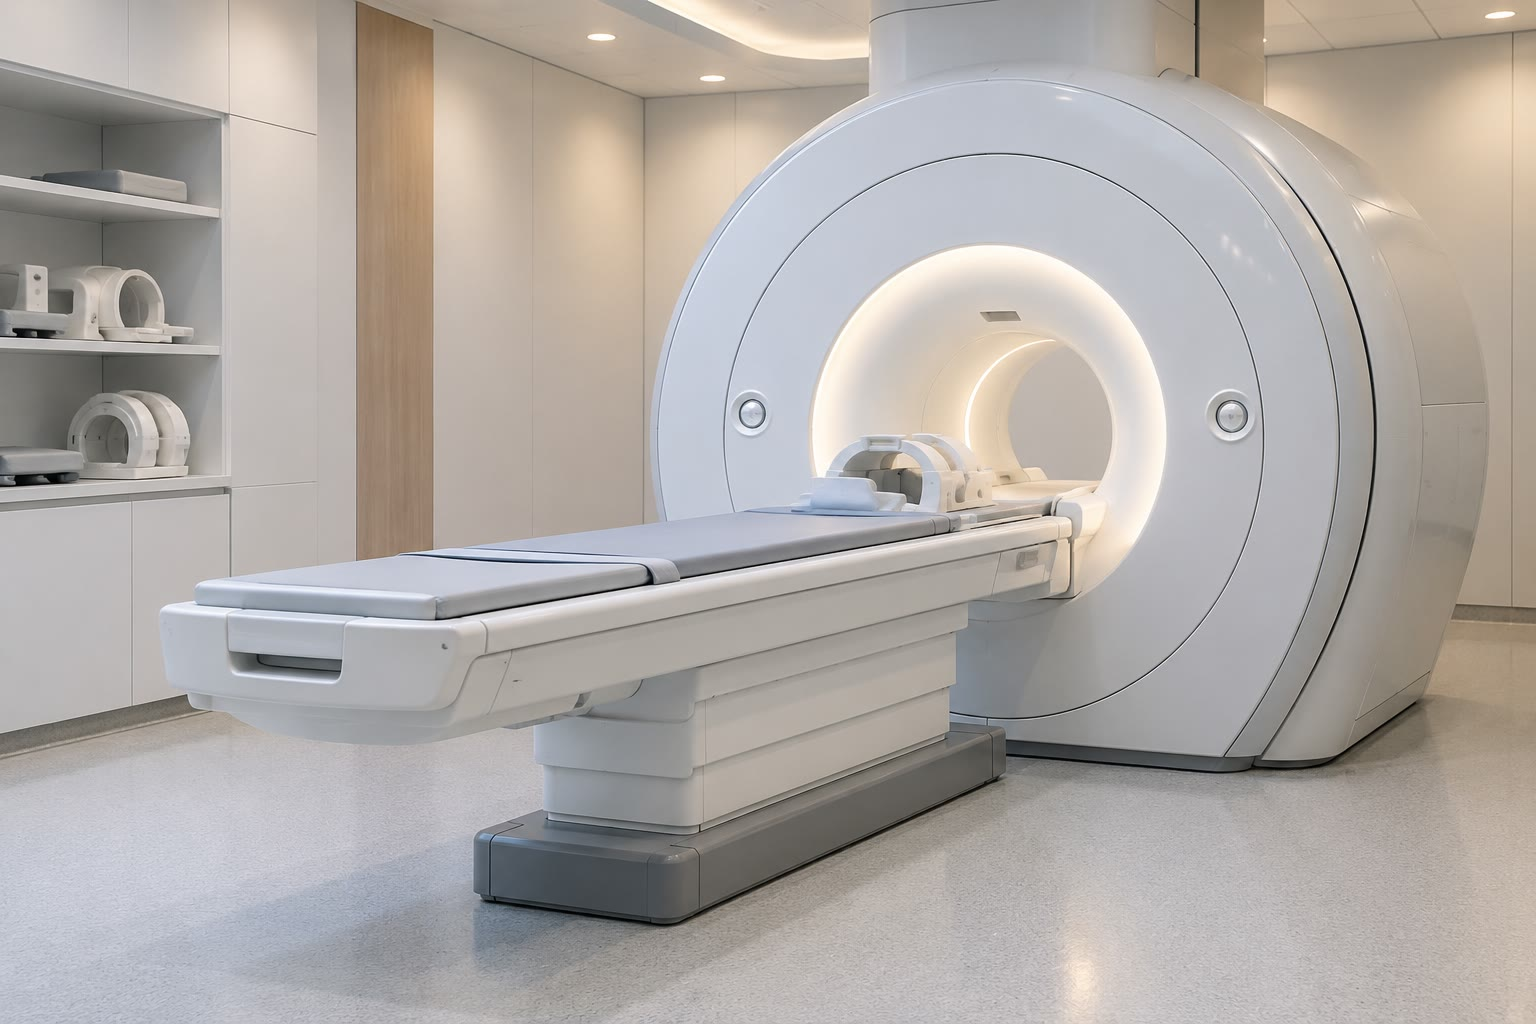
\includegraphics[width=0.52\linewidth]{images/book4/ai/b3-08-mri.jpg}\hspace{0.8em}%
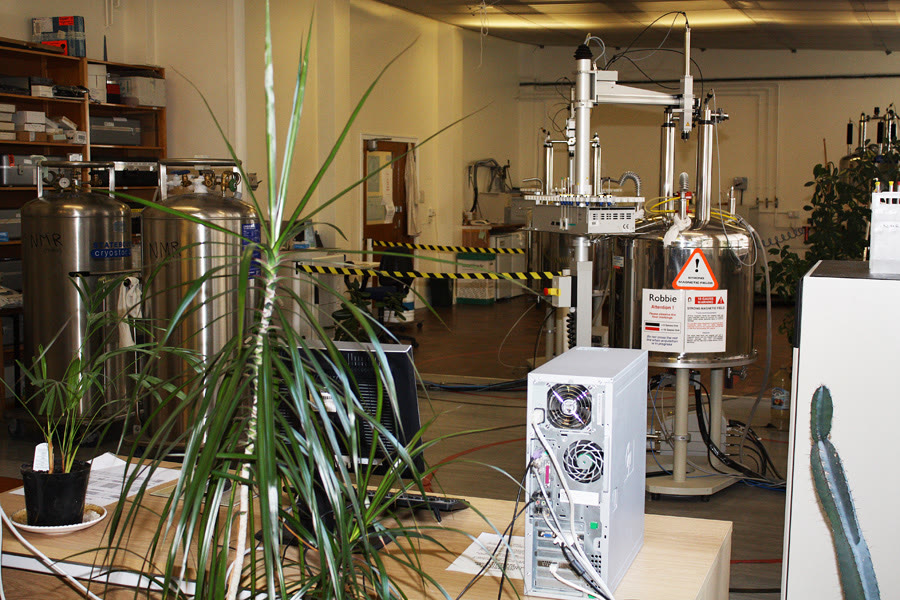
\includegraphics[width=0.4\linewidth]{images/book4/nmr-lab.jpg}

{\small 左：医院的 MRI 扫描仪。右：NMR 实验室；每台超导磁体
均置于其低温恒温器中，并定期补充左侧杜瓦瓶中的液氦
与液氮。照片：Shandchem，
CC BY 2.0.}
\end{omfigure}

\section{磁场中的核自旋}

\begin{definition}[核自旋量子数，旋磁比]\label{def:b3:advanced-nmr:nuclear-spin}
原子核具有自旋角动量，其量子数为 $I$，
称为\emph{核自旋量子数}\index{核自旋量子数}（$I = 0$
对应 \ce{^{12}C}、\ce{^{16}O}；$\frac12$ 对应 \ce{^1H}、\ce{^{13}C}、\ce{^{15}N}、\ce{^{19}F}、
\ce{^{31}P}；1 对应 \ce{^2H}、\ce{^{14}N}），并具有磁矩 $\boldsymbol\mu = \gamma\hat{\mathbf
I}$，与之成正比；$\gamma$ 为\emph{旋磁比}\index{旋磁比}。
沿磁场 $B_0$（取 $z$ 轴）方向，$\hat I_z$ 取值为 $m_I\hbar$，
$m_I = -I, \dots, I$。
\end{definition}

\begin{proposition}[塞曼能级]\label{prop:b3:advanced-nmr:zeeman}
在磁场 $B_0$ 中，能级为 $E_m = -m_I\gamma\hbar B_0$；跃迁 $\Delta m_I = \pm1$
所吸收的频率为
\[
\nu_0 = \frac{\gamma B_0}{2\pi}.
\]
\end{proposition}

\begin{proof}
$E = -\boldsymbol\mu\cdot\mathbf B = -\gamma B_0\hat I_z$，其本征值为 $-\gamma B_0m_I\hbar$。相邻
能级之差为 $\gamma\hbar B_0 = h\nu_0$。
\end{proof}

\begin{definition}[拉莫尔频率]\label{def:b3:advanced-nmr:larmor}
$\nu_0 = \gamma B_0/2\pi$ 为该核的\emph{拉莫尔频率}\index{拉莫尔频率}，
即共振频率，也是其磁矩
绕磁场进动的频率。
\end{definition}

\begin{example}[常见原子核]\label{ex:b3:advanced-nmr:nuclei}
% ledger: const:gammaP, nuc:C13.mu, nuc:F19.mu, nuc:P31.mu, nuc:N15.mu, const:muN
对于自旋 $\frac12$ 的原子核，若磁矩为 $\mu$，则 $\gamma/2\pi = \mu/(Ih) = 2\mu/h$。采用
实测磁矩：\ce{^1H} \qty{42.58}{MHz/T}，\ce{^{19}F} \qty{40.08}{MHz/T}，\ce{^{31}P}
\qty{17.25}{MHz/T}，\ce{^{13}C} \qty{10.71}{MHz/T}，\ce{^{15}N} \qty{-4.32}{MHz/T}。一台
“\qty{400}{MHz} 谱仪”的磁场为 $B_0 = \qty{9.4}{T}$，其质子
共振于 \qty{400.2}{MHz}，碳核共振于 \qty{100.7}{MHz}。
\end{example}

\begin{proposition}[能级布居的微小差异]\label{prop:b3:advanced-nmr:populations}
对于自旋 $\frac12$ 的原子核，在温度 $T$ 下，低能级上原子核的过量为
\[
\frac{N_\alpha - N_\beta}{N} \approx \frac{\gamma\hbar B_0}{2kT}.
\]
\end{proposition}

\begin{proof}
$N_\beta/N_\alpha = \eu^{-\Delta E/kT} \approx 1 - \Delta E/kT$，因 $\Delta E \ll kT$，故
$(N_\alpha - N_\beta)/(N_\alpha + N_\beta) \approx \Delta E/2kT$，其中 $\Delta E = \gamma\hbar B_0$。
\end{proof}

对于 \qty{9.4}{T} 磁场中、\qty{300}{K} 下的质子，过量为 \num{3.2e-5}，即每十万个
原子核中仅有 3 个参与贡献。由于过量与线圈中感生的
电压均随 $\gamma$ 和 $B_0$ 增大，
信号大致按 $\gamma^3B_0^2$ 增长，这既是磁体不断增强的原因，
也是 $\gamma$ 小、天然丰度低的原子核灵敏度低的原因，例如
\ce{^{13}C}。

\section{脉冲与自由感应衰减}

\begin{definition}[净磁化强度，旋转坐标系]\label{def:b3:advanced-nmr:magnetisation}
样品的\emph{净磁化强度}\index{净磁化强度} $\mathbf M$ 是
单位体积内核磁矩之和；平衡时，
其值为 $M_0$，方向沿 $\mathbf B_0$。\emph{旋转坐标系}\index{旋转坐标系}是一组
坐标轴 $x'$、$y'$、$z$，绕 $z$ 轴以所施加无线电波的频率转动；
在其中，$\nu_0$ 处的进动看上去减慢为偏移量 $\nu_0 -
\nu_{\mathrm{rf}}$。
\end{definition}

\begin{proposition}[进动]\label{prop:b3:advanced-nmr:precession}
处于磁场中的磁化强度满足 $\dd\mathbf M/\dd t = \gamma\,\mathbf M\times\mathbf B$；在
静磁场 $B_0\mathbf e_z$ 中，其横向分量绕 $z$ 轴以角
频率 $\omega_0 = \gamma B_0$ 转动，而 $M_z$ 保持不变。
\end{proposition}

\begin{proof}[部分证明]
该方程是具有角动量的磁矩的经典力矩方程，
由物理学承认。取 $\mathbf B = B_0\mathbf e_z$，则 $\dot M_x = \gamma
B_0M_y$，$\dot M_y = -\gamma B_0M_x$，$\dot M_z = 0$，其解为 $M_x + \iu M_y \propto
\eu^{-\iu\gamma B_0t}$：即以 $\omega_0$ 转动（从 $+z$ 方向看，$\gamma > 0$ 时为顺时针）。
\end{proof}

\begin{definition}[射频脉冲，翻转角]\label{def:b3:advanced-nmr:pulse}
称\emph{射频脉冲}\index{射频脉冲}为一段短促的
无线电波，其频率 $\nu_{\mathrm{rf}} \approx \nu_0$，其磁场 $B_1$ 在
旋转坐标系中固定于 $x'$ 方向，使 $\mathbf M$ 绕 $x'$ 转动。所转过的角度称为
\emph{翻转角}\index{翻转角} $\theta = \gamma B_1t_p$，对于持续时间为
$t_p$ 的脉冲：$90^\circ$ 脉冲使 $\mathbf M$ 落入 $x'y'$ 平面，$180^\circ$ 脉冲使之
反向。
\end{definition}

\begin{omfigure}
\tdplotsetmaincoords{70}{120}
\begin{tikzpicture}[tdplot_main_coords, font=\small, >=Stealth]
  \begin{scope}
    \draw[->, gray] (0,0,0) -- (1.8,0,0) node[anchor=north east] {$x'$};
    \draw[->, gray] (0,0,0) -- (0,1.8,0) node[anchor=north west] {$y'$};
    \draw[->, gray] (0,0,0) -- (0,0,1.8) node[anchor=south] {$z$, $\mathbf B_0$};
    \draw[->, omThm, very thick] (0,0,0) -- (0,0,1.4) node[anchor=west] {$\mathbf M$};
    \node[anchor=north] at (0,0,-0.9) {平衡};
  \end{scope}
  \begin{scope}[shift={(0,4.6,0)}]
    \draw[->, gray] (0,0,0) -- (1.8,0,0) node[anchor=north east] {$x'$};
    \draw[->, gray] (0,0,0) -- (0,1.8,0) node[anchor=north west] {$y'$};
    \draw[->, gray] (0,0,0) -- (0,0,1.8) node[anchor=south] {$z$};
    \draw[->, omDef, thick] (0,0,0) -- (1.2,0,0) node[anchor=south east, xshift=-2pt] {$\mathbf B_1$};
    \draw[->, omThm, very thick] (0,0,0) -- (0,1.4,0) node[anchor=south west] {$\mathbf M$};
    \node[anchor=north] at (0,0,-0.9) {$90^\circ_{x'}$ 脉冲之后};
  \end{scope}
  \begin{scope}[shift={(0,9.2,0)}]
    \draw[->, gray] (0,0,0) -- (1.8,0,0) node[anchor=north east] {$x'$};
    \draw[->, gray] (0,0,0) -- (0,1.8,0) node[anchor=north west] {$y'$};
    \draw[->, gray] (0,0,0) -- (0,0,1.8) node[anchor=south] {$z$};
    \draw[->, omThm, very thick] (0,0,0) -- (0,0,-1.4) node[anchor=west] {$\mathbf M$};
    \node[anchor=north] at (0,0,-1.6) {$180^\circ_{x'}$ 脉冲之后};
  \end{scope}
\end{tikzpicture}

{\small 旋转坐标系中的磁化强度。$90^\circ$ 脉冲绕 $x'$ 轴
使 $\mathbf M$ 由 $z$ 转至 $y'$（$\gamma > 0$ 时，转动遵循
绕 $\mathbf B_1$ 的左手定则，这是通常的约定）；$180^\circ$ 脉冲
使其反向。}
\end{omfigure}

\begin{definition}[自由感应衰减]\label{def:b3:advanced-nmr:fid}
经 $90^\circ$ 脉冲后，横向磁化强度以拉莫尔
频率进动，并在包围样品的线圈中感生出振荡电压，
该电压随磁化强度弛豫而衰减，称为\emph{自由感应
衰减}\index{自由感应衰减}（FID）。
\end{definition}

\begin{theorem}[由 FID 到谱]\label{thm:b3:advanced-nmr:lorentzian}
衰减振荡 $\eu^{-t/T_2}\cos(2\pi\nu t)$（$t \ge 0$）的傅里叶变换在
$\nu$ 附近是一条半高全宽为 $1/(\pi T_2)$ 的洛伦兹线。
\end{theorem}

\begin{proof}
写出信号 $\eu^{-t/T_2}\eu^{2\pi\iu\nu t}$ 并积分：
$\int_0^\infty\eu^{-t/T_2}\eu^{2\pi\iu(\nu - f)t}\dd t = \frac{1}{1/T_2 - 2\pi\iu(\nu - f)}$，其实部为
$\frac{T_2}{1 + 4\pi^2T_2^2(f - \nu)^2}$。它在 $f = \nu$ 处取最大值，并降至
一半，当 $2\pi T_2|f - \nu| = 1$ 时，即 $f - \nu = \pm1/(2\pi T_2)$：全宽
为 $1/(\pi T_2)$。
\end{proof}

\begin{omfigure}
\begin{tikzpicture}
\begin{axis}[name=fid, width=0.5\linewidth, height=4.6cm, xmin=0, xmax=0.4,
  ymin=-2.1, ymax=2.1, axis lines=left, xlabel={$t$ / s}, ylabel={信号},
  ytick=\empty, scaled x ticks=false, xticklabel style={/pgf/number format/fixed},
  tick label style={font=\small}, label style={font=\small}, title={\small 自由感应衰减}]
\addplot[omDef] table[x=t, y=s] {figdata/out/bachelor-3-nmr-fid.dat};
\addplot[gray, dashed, domain=0:0.4, samples=60] {2*exp(-x/0.1)};
\end{axis}
\begin{axis}[at={(fid.east)}, anchor=west, xshift=1.2cm, width=0.45\linewidth,
  height=4.6cm, xmin=0, xmax=350, ymin=-0.1, ymax=1.1, axis x line=bottom,
  axis y line=none, xlabel={偏移量 / Hz}, tick label style={font=\small},
  label style={font=\small}, title={\small 谱（傅里叶变换）}]
\addplot[omThm, thick] table[x=f, y=I] {figdata/out/bachelor-3-nmr-fid-spectrum.dat};
\end{axis}
\end{tikzpicture}

{\small 左：两条谱线的 FID（偏移量为 100 与 \qty{250}{Hz}，$T_2 = \qty{0.10}{s}$），
两个频率在指数包络内相互干涉而形成拍，
（虚线）。右：其傅里叶变换，为两条宽度为 \qty{3.2}{Hz} 的洛伦兹线。}
\end{omfigure}

\begin{proposition}[信号平均]\label{prop:b3:advanced-nmr:averaging}
将 $N$ 个 FID 相加，使信号增为 $N$ 倍，随机噪声增为 $\sqrt N$ 倍：
信噪比按 $\sqrt N$ 增长。
\end{proposition}

\begin{proof}
信号相干相加。独立采集的噪声的
均值为零，各自方差为 $\sigma^2$；$N$ 个独立项之和的方差为
$N\sigma^2$（见本科二年级分册中的误差传播律），因此其标准差
为 $\sqrt N\sigma$。
\end{proof}

DEPT 按所连氢原子数对 ${}^{13}$C 信号进行分类，
对质子和碳施加一系列脉冲，脉冲之间相隔
$1/2J$ 的延迟：质子的大磁化强度转移到碳上，
经单键耦合，使碳信号增强约
$\gamma_H/\gamma_C \approx 4$，末端质子脉冲的角度使 CH、\ce{CH2} 与
\ce{CH3} 的权重各不相同。同一思想——通过耦合在原子核之间转移磁化强度——
是下文二维实验的基础。

\section{弛豫}

\begin{definition}[纵向与横向弛豫时间]\label{def:b3:advanced-nmr:relaxation}
扰动之后 $M_z$ 回到 $M_0$ 呈指数规律，特征时间为
\emph{纵向弛豫时间}\index{纵向弛豫时间} $T_1$（自旋–晶格弛豫：能量传给外界）。
横向磁化强度衰减到零同样呈指数规律，
特征时间为
\emph{横向弛豫时间}\index{横向弛豫时间} $T_2 \le T_1$
（自旋–自旋弛豫：自旋之间相位相干性的丧失）。
\end{definition}

\begin{proposition}[反转恢复]\label{prop:b3:advanced-nmr:inversion-recovery}
施加 $180^\circ$ 脉冲后，$M_z(t) = M_0(1 - 2\eu^{-t/T_1})$，它在
$t_{\mathrm{null}} = T_1\ln2$ 处经过零点。
\end{proposition}

\begin{proof}
由弛豫方程 $\dd M_z/\dd t = (M_0 - M_z)/T_1$，初值 $M_z(0) = -M_0$，
解得 $M_0 - 2M_0\eu^{-t/T_1}$，当 $\eu^{-t/T_1} = \frac12$ 时该式为零。
\end{proof}

\begin{method}[测量 $T_1$ 并设定定量循环延迟]\label{met:b3:advanced-nmr:t1}
\begin{enumerate}
  \item 对一系列延迟运行脉冲序列 $180^\circ$--$\tau$--$90^\circ$--采集，
        其中 $\tau$ 取一系列值，每两次扫描之间至少等待 $5T_1$。
  \item 将每个信号拟合为 $M_0(1 - 2\eu^{-\tau/T_1})$，或读取零点，由此得 $T_1 =
        t_{\mathrm{null}}/\ln2$。
  \item 若用 $90^\circ$ 脉冲进行定量积分，两次扫描之间须至少等待弛豫最慢原子核的
        $5T_1$，此时缺失的磁化强度占比 $\eu^{-5} < 1\,\%$，
        可以忽略。
\end{enumerate}
\end{method}

\begin{omfigure}
\begin{tikzpicture}
\begin{axis}[width=0.62\linewidth, height=5cm, xmin=0, xmax=10, ymin=-1.1, ymax=1.15,
  axis lines=left, xlabel={$t$ / s}, ylabel={$M/M_0$}, legend cell align=left,
  legend style={font=\small, draw=none, at={(0.97,0.05)}, anchor=south east},
  tick label style={font=\small}, label style={font=\small}]
\addplot[omDef, thick] table[x=t, y=mz] {figdata/out/bachelor-3-nmr-relaxation.dat};
\addlegendentry{$M_z$ 经 $180^\circ$ 脉冲后（$T_1 = \qty{2.0}{s}$）}
\addplot[omThm, thick, dashed] table[x=t, y=mxy] {figdata/out/bachelor-3-nmr-relaxation.dat};
\addlegendentry{$M_{xy}$ 经 $90^\circ$ 脉冲后（$T_2 = \qty{0.5}{s}$）}
\addplot[gray, dotted, domain=0:10] {0};
\addplot[only marks, mark=*, mark size=1.5pt, black] coordinates {(1.386,0)};
\node[font=\small, anchor=north west] at (axis cs:1.5,-0.04) {$T_1\ln2$};
\end{axis}
\end{tikzpicture}

{\small 弛豫（模型值）。反转后的纵向磁化强度
在 $T_1\ln2$ 处恢复过零点；横向磁化强度
衰减更快，由 $T_2$ 决定。}
\end{omfigure}

\begin{definition}[自旋回波]\label{def:b3:advanced-nmr:echo}
在脉冲序列 $90^\circ$--$\tau$--$180^\circ$--$\tau$ 中，
因磁场不均匀而相位散开的自旋在时刻 $2\tau$ 重新聚焦，形成
\emph{自旋回波}\index{自旋回波}；其幅度按真实的 $T_2$ 衰减，
不受磁体不均匀性的影响。
\end{definition}

\begin{definition}[核欧沃豪斯效应]\label{def:b3:advanced-nmr:noe}
对一个自旋进行饱和或扰动，通过二者之间的偶极弛豫，
改变空间上邻近的另一自旋信号的强度，
即\emph{核欧沃豪斯效应}\index{核欧沃豪斯效应}（NOE）。
其增长速率与 $r^{-6}$ 成正比，因此只有在
相距约 \qty{0.5}{nm} 以内的原子核之间才能观察到，无论是否成键。
\end{definition}

\section{二维核磁共振}

\begin{definition}[二维谱、交叉峰、对角峰]\label{def:b3:advanced-nmr:two-d}
\emph{二维谱}\index{二维谱}通过重复一个脉冲序列记录，
该序列在采集时间之前带有递增的延迟 $t_1$，
采集时间为 $t_2$；经二重傅里叶变换，得到强度随两个频率变化的图谱。
\emph{交叉峰}\index{交叉峰}位于 $(\delta_1,
\delta_2)$ 表明 $\delta_1$ 与 $\delta_2$ 处的原子核相连（通过耦合或
邻近关系）；\emph{对角峰}\index{对角峰}位于 $(\delta, \delta)$，
对应单个原子核。
\end{definition}

\begin{definition}[COSY, HSQC, HMBC, NOESY]\label{def:b3:advanced-nmr:experiments}
\emph{COSY}\index{COSY}（相关谱）使相互耦合的质子相关联，
通常经三个键（H--C--C--H）相连。\emph{HSQC}\index{HSQC}
（异核单量子相干）使每个碳与
其直接相连的质子相关联。\emph{HMBC}\index{HMBC}（异核
多键相关）使碳与相隔两个或三个键的质子相关，
并跨越季碳和杂原子。\emph{NOESY}\index{NOESY}
使空间上相近的质子通过核欧沃豪斯效应相关联。
\end{definition}

\begin{omfigure}
\begin{tikzpicture}[font=\small]
  \foreach \y/\name in {3.2/{单脉冲}, 2.0/{反转恢复}, 0.8/{自旋回波}, -0.4/{COSY}}{
    \draw (0,\y) -- (9.3,\y); \node[anchor=east] at (-0.1,\y+0.25) {\name};}
  % one pulse
  \fill[black] (0.4,3.2) rectangle (0.6,3.75);
  \draw[omDef, domain=0:3.5, samples=120] plot (0.7+\x, {3.2+0.4*exp(-\x/1.2)*sin(\x*500)});
  % inversion recovery
  \fill[black] (0.4,2.0) rectangle (0.8,2.55); \node[font=\scriptsize] at (0.6,2.7) {180};
  \draw[<->] (0.85,1.85) -- (2.4,1.85) node[midway, below, font=\scriptsize] {$\tau$};
  \fill[black] (2.45,2.0) rectangle (2.65,2.55); \node[font=\scriptsize] at (2.55,2.7) {90};
  \draw[omDef, domain=0:3.0, samples=120] plot (2.75+\x, {2.0+0.4*exp(-\x/1.0)*sin(\x*500)});
  % spin echo
  \fill[black] (0.4,0.8) rectangle (0.6,1.35); \node[font=\scriptsize] at (0.5,1.5) {90};
  \draw[<->] (0.65,0.65) -- (2.4,0.65) node[midway, below, font=\scriptsize] {$\tau$};
  \fill[black] (2.45,0.8) rectangle (2.85,1.35); \node[font=\scriptsize] at (2.65,1.5) {180};
  \draw[<->] (2.9,0.65) -- (4.65,0.65) node[midway, below, font=\scriptsize] {$\tau$};
  \draw[omDef, domain=-1.2:2.5, samples=150] plot (4.65+\x, {0.8+0.35*exp(-abs(\x)/0.35)*cos(\x*700)});
  % COSY
  \fill[black] (0.4,-0.4) rectangle (0.6,0.15); \node[font=\scriptsize] at (0.5,0.3) {90};
  \draw[<->] (0.65,-0.55) -- (2.4,-0.55) node[midway, below, font=\scriptsize] {$t_1$（递增）};
  \fill[black] (2.45,-0.4) rectangle (2.65,0.15); \node[font=\scriptsize] at (2.55,0.3) {90};
  \draw[omDef, domain=0:3.0, samples=120] plot (2.75+\x, {-0.4+0.4*exp(-\x/1.0)*sin(\x*500)});
  \node[font=\scriptsize, anchor=west] at (5.9,-0.2) {采集（$t_2$）};
\end{tikzpicture}

{\small 脉冲序列（时间向右；实心方框为脉冲，
标注其翻转角（以度计）；蓝色为记录的信号）。自旋回波
峰位于第一个脉冲之后 $2\tau$ 处。}
\end{omfigure}

\begin{method}[借助二维谱解析结构]\label{met:b3:advanced-nmr:solve-2d}
\begin{enumerate}
  \item 由分子式、${}^1$H 积分和 ${}^{13}$C/DEPT 谱，列出
        CH、\ce{CH2}、\ce{CH3} 和季碳。
  \item HSQC：将每个质子信号归属到与其相连的碳上。
  \item COSY：将连有质子的碳连成自旋体系（
        相邻碳构成的链）。
  \item HMBC：跨越季碳、羰基和杂原子连接各自旋体系，
        在 COSY 无信号处。
  \item NOESY：借助穿越空间的接触，确定相对
        构型与构象。
  \item 将每个信号与所提出的结构逐一核对。
\end{enumerate}
\end{method}

\begin{omfigure}
\begin{tikzpicture}
\begin{axis}[name=cosy, width=0.47\linewidth, height=0.47\linewidth, x dir=reverse,
  y dir=reverse, xmin=0.5, xmax=4.6, ymin=0.5, ymax=4.6, axis lines=box,
  xlabel={质子化学位移 $\delta_{\mathrm H}$ / ppm}, ylabel={质子化学位移 $\delta_{\mathrm H}$ / ppm},
  tick label style={font=\small}, label style={font=\small}, title={\small COSY}]
\addplot[gray, dotted, domain=0.5:4.6] {x};
\addplot[only marks, mark=*, mark size=2.2pt, black] table[x=h1, y=h2] {figdata/out/bachelor-3-nmr-2d-cosy-diag.dat};
\addplot[only marks, mark=*, mark size=2.2pt, omThm] table[x=h1, y=h2] {figdata/out/bachelor-3-nmr-2d-cosy-cross.dat};
\end{axis}
\begin{axis}[at={(cosy.east)}, anchor=west, xshift=1.3cm, width=0.47\linewidth,
  height=0.47\linewidth, x dir=reverse, y dir=reverse, xmin=0.5, xmax=4.6,
  ymin=0, ymax=185, axis lines=box, xlabel={质子化学位移 $\delta_{\mathrm H}$ / ppm},
  ylabel={碳化学位移 $\delta_{\mathrm C}$ / ppm}, tick label style={font=\small},
  label style={font=\small}, title={\small HSQC（蓝色）和 HMBC（红色）}]
\addplot[only marks, mark=square*, mark size=2.2pt, omDef] table[x=h, y=c] {figdata/out/bachelor-3-nmr-2d-hsqc.dat};
\addplot[only marks, mark=o, mark size=2.6pt, omThm, thick] table[x=h, y=c] {figdata/out/bachelor-3-nmr-2d-hmbc.dat};
\end{axis}
\end{tikzpicture}

{\small 丁酸乙酯 \ce{CH3CH2CH2COOCH2CH3} 的二维谱，
按实测化学位移绘制。COSY：黑色为对角峰；红色为
相邻碳上质子之间的交叉峰——两个自旋体系，乙基与
丙基，酯氧两侧无交叉峰。右图：HSQC 峰
（方块）将每个质子与其所连的碳相连；HMBC 峰（圆圈）显示 OCH$_2$
质子（\qty{4.13}{ppm}）与 CH$_2$C=O 质子（\qty{2.28}{ppm}）均
与位于 \qty{173.6}{ppm} 处的羰基碳相关。}
\end{omfigure}

\section{其他原子核与动力学}

氟-19 和磷-31 的自旋为 $\frac12$，丰度达 100\,\%，
旋磁比 $\gamma$ 较大，观测难度几乎与质子相当；其化学位移范围宽，
使它们成为探测周围环境的精确探针（药物、磷酸盐、配体，例如
在\cref{ch:b3:organometallic-bonding}中的膦类配体）。氮-15 丰度低、
信号弱，通常通过与之相连的质子间接观测。
不同原子核之间的耦合可通过去耦消除，
与本科二年级分册中对 ${}^{13}$C 的处理相同。

\begin{definition}[聚并温度]\label{def:b3:advanced-nmr:coalescence}
当一个原子核在两种化学位移
相差 $\Delta\nu$（以赫兹计）的环境之间交换时，其两条谱线随交换加快而展宽，
最终在\emph{聚并温度}\index{聚并温度}
$T_c$ 下合并为一条。
\end{definition}

\begin{proposition}[聚并时的速率]\label{prop:b3:advanced-nmr:coalescence}
对两个布居数相等且无耦合的位点，聚并时的交换速率常数
为 $k_c = \pi\Delta\nu/\sqrt2$。
\end{proposition}
\admitted

由含交换项的布洛赫方程导出的过程将在更
高级课程中讨论。借助艾林方程（见\cref{ch:b3:rate-theories}），
即可由速率求得能垒：动态核磁共振可测定酰胺键的旋转、环翻转
及配体交换的能垒，为 40 至 \qty{100}{kJ/mol}。

\begin{example}[一幅 MRI 图像]\label{ex:b3:advanced-nmr:mri}
在磁共振成像中，场梯度使水质子的拉莫尔频率
随位置而变，因此信号的傅里叶变换
即为显示其位置的图像。对比度来自弛豫：
重复时间与回波延迟的选取，使图像
按 $T_1$ 或 $T_2$ 加权，二者在不同组织间各不相同；含钆
造影剂可缩短附近水的 $T_1$（见\cref{ch:b3:bioinorganic}）。
\end{example}

\begin{inthelab}[准备谱仪]
将溶于氘代溶剂的样品放入探头。
谱仪锁定氘信号，以补偿磁场的缓慢漂移；
探头需对每种原子核的频率进行调谐与匹配；
通过调节匀场线圈，使样品区域内磁场均匀，
直至谱线变窄。磁铁的磁场始终存在：钢制工具、
信用卡和心脏起搏器须放在标记的安全线之外。
\end{inthelab}

\begin{history}[从共振到二维谱]
费利克斯·布洛赫和爱德华·珀塞尔于 1946 年
在宏观物质中探测到核磁共振（1952 年诺贝尔物理学奖）。理查德·恩斯特
于 1966 年引入脉冲傅里叶变换核磁共振，
受让·耶纳思想的启发，于 20 世纪 70 年代提出二维谱学（1991 年诺贝尔化学奖）。
\end{history}

\section{练习}

\begin{exercise}[$\star$]\label{exo:b3:advanced-nmr:1}
% ledger: const:gammaP, nuc:C13.mu, nuc:F19.mu
计算 \ce{^1H}、\ce{^{13}C} 和 \ce{^{19}F} 在 \qty{14.1}{T}
下的拉莫尔频率（$\gamma/2\pi = 42.58$、10.71 和 \qty{40.08}{MHz/T}）。
\end{exercise}

\begin{exercise}[$\star$]\label{exo:b3:advanced-nmr:2}
计算在 \qty{9.4}{T} 和
\qty{300}{K} 下低能级中质子的相对过量。温度降至 \qty{4}{K} 时，它改变多少？
\end{exercise}

\begin{exercise}[$\star$]\label{exo:b3:advanced-nmr:3}
对质子，$90^\circ$ 脉冲持续 \qty{10}{\micro s}。$\gamma B_1/2\pi$ 为多少？
$180^\circ$ 脉冲持续多长？\qty{5}{\micro s} 脉冲会产生什么效果？
\end{exercise}

\begin{exercise}[$\star$]\label{exo:b3:advanced-nmr:4}
谱线在半高处的宽度为 \qty{3.2}{Hz}。假设磁场完全
均匀，求 $T_2$ 为多少？
\end{exercise}

\begin{exercise}[$\star\star$]\label{exo:b3:advanced-nmr:5}
% ledger: iso:C13
利用每个核的信号 $\propto\gamma^3$ 以及
\ce{^{13}C} 的 1.1\,\% 天然丰度，比较 ${}^{13}$C 与 ${}^1$H 核磁共振的灵敏度。
在相同信噪比下，${}^{13}$C 谱需要多出多少次扫描？
\end{exercise}

\begin{exercise}[$\star\star$]\label{exo:b3:advanced-nmr:6}
在反转恢复实验中，某碳的信号在
$\tau = \qty{1.39}{s}$ 时消失。求 $T_1$ 及定量测定所需的循环延迟。
\end{exercise}

\begin{exercise}[$\star\star$]\label{exo:b3:advanced-nmr:7}
在丁酮 \ce{CH3COCH2CH3} 的 COSY 谱中，出现哪些交叉峰？
哪些碳显示出来自单峰甲基质子的 HMBC 峰？
\end{exercise}

\begin{exercise}[$\star\star$]\label{exo:b3:advanced-nmr:8}
某酰胺的两个甲基信号在低温下相距 \qty{50}{Hz}，
在 \qty{330}{K} 时合并。计算合并时的交换速率，
并利用 $\Delta G^\ddagger = RT_c\ln(k_BT_c/hk_c)$ 求活化吉布斯自由能。
\end{exercise}

\begin{exercise}[$\star\star$]\label{exo:b3:advanced-nmr:9}
质子 H$_a$ 与 H$_b$ 之间的 NOE 比 H$_a$ 与 H$_c$ 之间的强四倍，
后者的距离为 \qty{0.30}{nm}。估算 H$_a$--H$_b$ 的距离。
\end{exercise}

\begin{exercise}[$\star\star\star$]\label{exo:b3:advanced-nmr:10}
试在旋转坐标系中求解 $\dd\mathbf M/\dd t = \gamma\mathbf M\times\mathbf B_1$，
设 $\mathbf B_1$ 沿 $x'$ 方向，证明脉冲使 $\mathbf M$ 转过 $\gamma B_1t_p$，转轴为 $x'$。
\end{exercise}

\begin{exercise}[$\star\star\star$]\label{exo:b3:advanced-nmr:11}
解释为何自旋回波能重聚由非均匀
磁场引起的失相，却不能重聚由自旋间随机相互作用引起的失相。
回波振幅测量的是哪一个时间常数？
\end{exercise}

\begin{exercise}[$\star\star\star$]\label{exo:b3:advanced-nmr:12}
推断化合物 \ce{C4H8O2} 的结构，其 ${}^1$H 谱中出现一个
四重峰（2H，4.12 ppm）、一个单峰（3H，2.05 ppm）和一个三重峰（3H，
1.26 ppm），其 HMBC 谱显示四重峰的质子与一个
171 ppm 处的碳存在相关（题中数据）。同分子式的其他哪种酯
会给出不同的 HMBC 图谱？不同之处何在？
\end{exercise}

\section{问题：二维谱中的菠萝酯}

\begin{problem}[{周末问题——再解丁酸乙酯，由二维谱出发：
由 COSY 确定自旋体系，由 HSQC 确定碳，
由 HMBC 确定酯键，并求定量碳谱所需的
循环延迟}]
\label{pb:b3:advanced-nmr:1}
% ledger: nmr:ethylbutanoate-OCH2, nmr:ethylbutanoate-CH2CO, nmr:ethylbutanoate-CH2, nmr:ethylbutanoate-OCH2CH3, nmr:ethylbutanoate-CH3, c13:ethylbutanoate.CO, c13:ethylbutanoate.OCH2, c13:ethylbutanoate.CH2CO, c13:ethylbutanoate.CH2, c13:ethylbutanoate.OCH2CH3, c13:ethylbutanoate.CH3
一种具有菠萝香气的酯 \ce{C6H12O2}，其 ${}^1$H 信号位于 4.13（2H，
q）、2.28（2H，t）、1.66（2H，m）、1.25（3H，t）和 0.95 ppm（3H，t）处，${}^{13}$C 信号
位于 173.6、60.1、36.3、18.6、14.3 和 13.7 ppm，于 \qty{9.4}{T} 下测得。其二维
谱即第 4 节图中所示。本题数据：各碳的 $T_1$
值：羰基碳约为 \qty{20}{s}，其余碳为 2 至
\qty{6}{s}。

\medskip\noindent\textbf{第一部分——一维谱。}
\begin{enumerate}
  \item 计算 \ce{C6H12O2} 的不饱和度。
  \item 哪一个 ${}^{13}$C 信号属于羰基碳？哪一个属于与氧相连的碳？
  \item 有多少个连有质子的碳？DEPT-135 谱会显示什么？
  \item 在 \qty{9.4}{T} 下，${}^1$H 和 ${}^{13}$C 的拉莫尔频率各为多少？
  \item 四重峰的耦合常数为 \qty{7.2}{Hz}。以 ppm 计，该
        四重峰在 \qty{400}{MHz} 下的宽度是多少？
  \item 为什么仅凭一维谱无法确定片段的连接顺序？
\end{enumerate}

\medskip\noindent\textbf{第二部分——COSY。}
\begin{enumerate}[resume]
  \item 列出 COSY 谱图中的交叉峰。
  \item 推断两个自旋体系。
  \item 为什么 4.13 与 2.28 ppm 之间没有交叉峰？
  \item 哪一个质子信号与另外两个信号发生耦合？解释其峰的多重性。
  \item 0.95 与 1.25 ppm 之间若出现交叉峰，意味着什么？
  \item 画出两个片段。
\end{enumerate}

\medskip\noindent\textbf{第三部分——HSQC 与 HMBC。}
\begin{enumerate}[resume]
  \item 由 HSQC 谱，将每个碳指认到与其相连的质子。
  \item 哪两个甲基碳只能借助 HSQC 加以区分？
  \item 哪一个 HMBC 峰将乙基片段与羰基联系起来，经过
        几个化学键？
  \item 哪些 HMBC 峰将丙基片段与羰基联系起来？
  \item 推断其结构，并排除其同分异构体丙酸丙酯。
  \item 为什么通常观察不到跨越四个或更多化学键的 HMBC 峰？
\end{enumerate}

\medskip\noindent\textbf{第四部分——定量碳谱。}
\begin{enumerate}[resume]
  \item 为什么普通 ${}^{13}$C 谱的积分面积与碳原子数
        不成正比？
  \item 羰基碳能恢复其平衡磁化强度的几分之几，
        若每隔 \qty{5}{s} 以 $90^\circ$ 脉冲重复扫描
        （每次均从零开始）？
  \item 经过 $5T_1$ 后，恢复了几分之几？
  \item 除弛豫外，质子去偶的哪一效应会使碳的积分面积失真，
        该效应如何被抑制？
  \item 若延迟取 $5T_1$，256 次扫描需要多长时间？
  \item 给出结论：获得本酯定量 ${}^{13}$C 谱所需的最小
        循环延迟。
\end{enumerate}
\end{problem}
